% Options for packages loaded elsewhere
\PassOptionsToPackage{unicode}{hyperref}
\PassOptionsToPackage{hyphens}{url}
%
\documentclass[
]{article}
\title{Get and summarize AFSC survey data}
\author{Kirstin Holsman, Alaska Fisheries Science Center}
\date{}

\usepackage{amsmath,amssymb}
\usepackage{lmodern}
\usepackage{iftex}
\ifPDFTeX
  \usepackage[T1]{fontenc}
  \usepackage[utf8]{inputenc}
  \usepackage{textcomp} % provide euro and other symbols
\else % if luatex or xetex
  \usepackage{unicode-math}
  \defaultfontfeatures{Scale=MatchLowercase}
  \defaultfontfeatures[\rmfamily]{Ligatures=TeX,Scale=1}
\fi
% Use upquote if available, for straight quotes in verbatim environments
\IfFileExists{upquote.sty}{\usepackage{upquote}}{}
\IfFileExists{microtype.sty}{% use microtype if available
  \usepackage[]{microtype}
  \UseMicrotypeSet[protrusion]{basicmath} % disable protrusion for tt fonts
}{}
\makeatletter
\@ifundefined{KOMAClassName}{% if non-KOMA class
  \IfFileExists{parskip.sty}{%
    \usepackage{parskip}
  }{% else
    \setlength{\parindent}{0pt}
    \setlength{\parskip}{6pt plus 2pt minus 1pt}}
}{% if KOMA class
  \KOMAoptions{parskip=half}}
\makeatother
\usepackage{xcolor}
\IfFileExists{xurl.sty}{\usepackage{xurl}}{} % add URL line breaks if available
\IfFileExists{bookmark.sty}{\usepackage{bookmark}}{\usepackage{hyperref}}
\hypersetup{
  pdftitle={Get and summarize AFSC survey data},
  pdfauthor={Kirstin Holsman, Alaska Fisheries Science Center},
  hidelinks,
  pdfcreator={LaTeX via pandoc}}
\urlstyle{same} % disable monospaced font for URLs
\usepackage[margin=1in]{geometry}
\usepackage{color}
\usepackage{fancyvrb}
\newcommand{\VerbBar}{|}
\newcommand{\VERB}{\Verb[commandchars=\\\{\}]}
\DefineVerbatimEnvironment{Highlighting}{Verbatim}{commandchars=\\\{\}}
% Add ',fontsize=\small' for more characters per line
\usepackage{framed}
\definecolor{shadecolor}{RGB}{248,248,248}
\newenvironment{Shaded}{\begin{snugshade}}{\end{snugshade}}
\newcommand{\AlertTok}[1]{\textcolor[rgb]{0.94,0.16,0.16}{#1}}
\newcommand{\AnnotationTok}[1]{\textcolor[rgb]{0.56,0.35,0.01}{\textbf{\textit{#1}}}}
\newcommand{\AttributeTok}[1]{\textcolor[rgb]{0.77,0.63,0.00}{#1}}
\newcommand{\BaseNTok}[1]{\textcolor[rgb]{0.00,0.00,0.81}{#1}}
\newcommand{\BuiltInTok}[1]{#1}
\newcommand{\CharTok}[1]{\textcolor[rgb]{0.31,0.60,0.02}{#1}}
\newcommand{\CommentTok}[1]{\textcolor[rgb]{0.56,0.35,0.01}{\textit{#1}}}
\newcommand{\CommentVarTok}[1]{\textcolor[rgb]{0.56,0.35,0.01}{\textbf{\textit{#1}}}}
\newcommand{\ConstantTok}[1]{\textcolor[rgb]{0.00,0.00,0.00}{#1}}
\newcommand{\ControlFlowTok}[1]{\textcolor[rgb]{0.13,0.29,0.53}{\textbf{#1}}}
\newcommand{\DataTypeTok}[1]{\textcolor[rgb]{0.13,0.29,0.53}{#1}}
\newcommand{\DecValTok}[1]{\textcolor[rgb]{0.00,0.00,0.81}{#1}}
\newcommand{\DocumentationTok}[1]{\textcolor[rgb]{0.56,0.35,0.01}{\textbf{\textit{#1}}}}
\newcommand{\ErrorTok}[1]{\textcolor[rgb]{0.64,0.00,0.00}{\textbf{#1}}}
\newcommand{\ExtensionTok}[1]{#1}
\newcommand{\FloatTok}[1]{\textcolor[rgb]{0.00,0.00,0.81}{#1}}
\newcommand{\FunctionTok}[1]{\textcolor[rgb]{0.00,0.00,0.00}{#1}}
\newcommand{\ImportTok}[1]{#1}
\newcommand{\InformationTok}[1]{\textcolor[rgb]{0.56,0.35,0.01}{\textbf{\textit{#1}}}}
\newcommand{\KeywordTok}[1]{\textcolor[rgb]{0.13,0.29,0.53}{\textbf{#1}}}
\newcommand{\NormalTok}[1]{#1}
\newcommand{\OperatorTok}[1]{\textcolor[rgb]{0.81,0.36,0.00}{\textbf{#1}}}
\newcommand{\OtherTok}[1]{\textcolor[rgb]{0.56,0.35,0.01}{#1}}
\newcommand{\PreprocessorTok}[1]{\textcolor[rgb]{0.56,0.35,0.01}{\textit{#1}}}
\newcommand{\RegionMarkerTok}[1]{#1}
\newcommand{\SpecialCharTok}[1]{\textcolor[rgb]{0.00,0.00,0.00}{#1}}
\newcommand{\SpecialStringTok}[1]{\textcolor[rgb]{0.31,0.60,0.02}{#1}}
\newcommand{\StringTok}[1]{\textcolor[rgb]{0.31,0.60,0.02}{#1}}
\newcommand{\VariableTok}[1]{\textcolor[rgb]{0.00,0.00,0.00}{#1}}
\newcommand{\VerbatimStringTok}[1]{\textcolor[rgb]{0.31,0.60,0.02}{#1}}
\newcommand{\WarningTok}[1]{\textcolor[rgb]{0.56,0.35,0.01}{\textbf{\textit{#1}}}}
\usepackage{graphicx}
\makeatletter
\def\maxwidth{\ifdim\Gin@nat@width>\linewidth\linewidth\else\Gin@nat@width\fi}
\def\maxheight{\ifdim\Gin@nat@height>\textheight\textheight\else\Gin@nat@height\fi}
\makeatother
% Scale images if necessary, so that they will not overflow the page
% margins by default, and it is still possible to overwrite the defaults
% using explicit options in \includegraphics[width, height, ...]{}
\setkeys{Gin}{width=\maxwidth,height=\maxheight,keepaspectratio}
% Set default figure placement to htbp
\makeatletter
\def\fps@figure{htbp}
\makeatother
\setlength{\emergencystretch}{3em} % prevent overfull lines
\providecommand{\tightlist}{%
  \setlength{\itemsep}{0pt}\setlength{\parskip}{0pt}}
\setcounter{secnumdepth}{-\maxdimen} % remove section numbering
\ifLuaTeX
  \usepackage{selnolig}  % disable illegal ligatures
\fi

\begin{document}
\maketitle

{
\setcounter{tocdepth}{2}
\tableofcontents
}
\hypertarget{afsc-survey-cpue-data-github.comkholsmanafsc_cpue}{%
\paragraph{\texorpdfstring{\href{https://github.com/kholsman/AFSC_CPUE}{\textbf{AFSC
Survey CPUE data:
github.com/kholsman/AFSC\_CPUE}}}{AFSC Survey CPUE data: github.com/kholsman/AFSC\_CPUE}}\label{afsc-survey-cpue-data-github.comkholsmanafsc_cpue}}

Repo maintained by:\\
Kirstin Holsman\\
Alaska Fisheries Science Center\\
NOAA Fisheries, Seattle WA\\
\textbf{\url{kirstin.holsman@noaa.gov}}\strut \\
\emph{Last updated: Jan 05, 2023}

\hypertarget{overview}{%
\section{Overview}\label{overview}}

The below scripts return a list object cpue\_data saved as a compressed
Rdata file with the naming `reg.srvy\#.spp.cpue\_data.Rdata' such as
``ebs.srvy98.plk.cpue\_data.Rdata''. Each cpue\_data list contains 8
data.frames:

\begin{Shaded}
\begin{Highlighting}[]
\FunctionTok{load}\NormalTok{(}\StringTok{"data/out/2023\_01\_03/cpue/ebs/ebs.srvy98.plk.cpue\_data.Rdata"}\NormalTok{)}

\FunctionTok{names}\NormalTok{(cpue\_data)}
\end{Highlighting}
\end{Shaded}

\begin{verbatim}
## [1] "totalB_N_SEBS_NBS"      "totalB_N_SEBS"          "mnCPUE_strata_yr"      
## [4] "total_bin_B_N_SEBS"     "total_bin_B_N_SEBS_NBS" "mnCPUE_strata_bin_yr"  
## [7] "CPUE_station_bin_yr"    "CPUE_station_yr"
\end{verbatim}

The data.frames are

\begin{enumerate}
\def\labelenumi{\arabic{enumi}.}
\item
  \textbf{totalB\_N\_SEBS\_NBS}: Total biomass (kg) or abundance (\# of
  fish) for the species in each year for NEBS + SEBS survey results\\
\item
  \textbf{totalB\_N\_SEBS}: Total biomass (kg) or abundance (\# of fish)
  for the species in each year for only SEBS survey results
\item
  \textbf{mnCPUE\_strata\_yr} : Average survey CPUE (kg per Km2) or
  abundance (\# per Km2) for the species in each strata and year
\item
  \textbf{total\_bin\_B\_N\_SEBS}: Total biomass (kg) or abundance (\#
  of fish) for each bin (10 mm) for the species in each year for NEBS +
  SEBS survey results
\item
  \textbf{total\_bin\_B\_N\_SEBS\_NBS} : Total biomass (kg) or abundance
  (\# of fish) for each bin (10 mm) for the species in each year for
  only the SEBS survey results
\item
  \textbf{mnCPUE\_strata\_bin\_yr}: Average survey CPUE (kg per Km2) or
  abundance (\# per Km2) for each size bin for the species in each
  strata and year
\item
  \textbf{CPUE\_station\_bin\_yr}: Station specific survey CPUE (kg per
  Km2) or abundance (\# per Km2) for each size bin for the species in
  eachyear
\item
  \textbf{CPUE\_station\_yr}: Station specific survey CPUE (kg per Km2)
  or abundance (\# per Km2) for the species in each year
\end{enumerate}

These are calculated from the RACEBASE data tables for survey results
where total CPUE was recorded for the species \(s\) (location\_catch) at
each haul, expanded to include stations \(i\) where CPUE=0 (location)
and expanded to each size bin \(l\) using the proportional subset of
frequency of fish of given length (mm), binned into 10 mm bins (\(l\))
and predicted weight (\(\hat{W}\)) for each size bin \(l\) at each
station \(i\):

\[B_{s,y} =  \bar{CPUE_{s,k,y}} \dot{}A_{k}\] where \(A_{k}\) is the
area of the strata \(k\) in \(Km^2\) and \(\bar{CPUE_{s,k,y}}\) is the
strata specific average CPUE (kg per \(Km^2\) or number per \(Km^2\)) of
all stations \(i\) in strata \(k\):
\[\bar{CPUE_{s,k,y}} = \frac{1}{n_k}\dot{}\sum_{n_k}{CPUE_{s,k,y,i}}\]
where \$ CPUE\_\{s,k,y,i\} \$ is the station specific CPUE (saves as the
object \texttt{cpue\_data\$CPUE\_station\_yr}).

To obtain population level estimates of the biomass or abundance of fish
by size bin \(l\), we used a length weight regression to esimate the
weight of each size fish \(j\) measured (\(\hat{W}\)) to calculate the
proportion by weight or frequency at each station where
\[\hat{W} = \alpha_s+L_j^{\beta_s} \]

and
\[p^w_{l,i} = \frac{N_{l,i}\dot{}\hat{\bar{W_{l,i}}}}{\sum_{}{N_{l,i}\dot{}\hat{\bar{W_{l,i}}}}}\]
and \[p^N_{l,i} = \frac{N_{l,i}}{\sum_{}{N_{l,i}}}\] This was then
multiplied by the CPUE at each station (\(CPUE_{s,k,y,i}\)) to obtain a
station estimate of CPUE by size bin \(l\)
\[CPUE_{s,k,y,l,i} = p^N_{l,i}\dot{}CPUE_{s,k,y,i}\]

Finally, the average strata CPUE (\(\bar{CPUE_{s,k,y,l}}\)) and whole of
EBS biomass by size bin (\(B_{s,y,l}\)) was calculated as:
\[\bar{CPUE_{s,k,y,l}} = \frac{1}{n_k}\dot{}\sum_{n_k}{CPUE_{s,k,y,l,i}}\]
and \[B_{s,y,l}= \bar{CPUE_{s,k,y,l}}\dot{}A_{k}\] \# Code\\
.

\hypertarget{step-0-set-up-the-r-workspace}{%
\subsection{Step 0: Set up the R
workspace}\label{step-0-set-up-the-r-workspace}}

The first step is to set up the switches for what files to update and
create in the file \texttt{R/setup.R}. The code below then loads these
settings as well as base data, functions, and packages.

\begin{Shaded}
\begin{Highlighting}[]
  \CommentTok{\# get everything set up:}
  \CommentTok{\#{-}{-}{-}{-}{-}{-}{-}{-}{-}{-}{-}{-}{-}{-}{-}{-}{-}{-}{-}{-}{-}{-}{-}{-}{-}{-}{-}{-}{-}{-}{-}{-}{-}{-}{-}{-}{-}{-}{-}{-}}
    \CommentTok{\# rm(list=ls())}
\CommentTok{\# this uses the password saved in R/password.R}
    \FunctionTok{suppressMessages}\NormalTok{(}\FunctionTok{source}\NormalTok{(}\StringTok{"R/make.R"}\NormalTok{))}
\end{Highlighting}
\end{Shaded}

\hypertarget{step-1-update-sql-queries-level1}{%
\subsection{Step 1: Update SQL queries
(level1)}\label{step-1-update-sql-queries-level1}}

This step must be run on a computer that has access to RACEBASE. The
code below will generate the base files for steps 2 and 3 below,and will
save them in the folder data/in/2023\_01\_03 under subfolders for each
region in \texttt{srvys\$reg} and each species in \texttt{splist} (see
\texttt{R/setup.R} to change these settings).

\textbf{IMPORTANT:}

\begin{itemize}
\item
  \textbf{This step must be run in 32 bit R (RODBC doesn't run in 64 bit
  R) and must be connected to the RACEBASE SQL database}
\item
  \textbf{To change R studio from the default 64 bit to 32 bit go to
  Tools\textgreater Global options and select the 32 bit version of R.}
\item
  \textbf{The code will connect to the SQL database using your password
  and username. Remember to update the \texttt{username\_path} in the
  first line of the \texttt{R/setup.R} file and corresponding
  \texttt{username} and \texttt{password} under
  \texttt{username\_password.R}. A template is available under
  \texttt{R/}.}
\end{itemize}

\begin{Shaded}
\begin{Highlighting}[]
  \CommentTok{\# update the SQL queries}
  \CommentTok{\#{-}{-}{-}{-}{-}{-}{-}{-}{-}{-}{-}{-}{-}{-}{-}{-}{-}{-}{-}{-}{-}{-}{-}{-}{-}{-}{-}{-}{-}{-}{-}{-}{-}{-}{-}{-}{-}{-}{-}{-}{-}{-}{-}{-}{-}  }
  \FunctionTok{source}\NormalTok{(}\FunctionTok{file.path}\NormalTok{(code.path,}\StringTok{"R/sub\_scripts/runRACE\_qrys.R"}\NormalTok{))}
\end{Highlighting}
\end{Shaded}

\hypertarget{step-2-update-the-lwa-regressions}{%
\subsection{Step 2: Update the LWA
regressions}\label{step-2-update-the-lwa-regressions}}

The default code for RACEBASE uses set LW relationships, however we
prefer to update the LW regressions using glms. Depending on how many
observations exist the LW relationships can be region specific or use
data across all regions.The default below is all regions combined. This
code generates two outputs in data/out/2023\_01\_03,
LWGlms\_srvy\_all\_regs.Rdata and \texttt{LW\_SmryTable.Rdata}. It also
updates the \texttt{species\_lkup\$LW\_a} and species\_lkup\$LW\_b`
parms used in Step 3.

\begin{Shaded}
\begin{Highlighting}[]
  \CommentTok{\# update the LW regressions }
  \CommentTok{\#{-}{-}{-}{-}{-}{-}{-}{-}{-}{-}{-}{-}{-}{-}{-}{-}{-}{-}{-}{-}{-}{-}{-}{-}{-}{-}{-}{-}{-}{-}{-}{-}{-}{-}{-}{-}{-}{-}{-}{-}{-}{-}{-}{-}{-}  }

  \ControlFlowTok{if}\NormalTok{(update\_LWdata}\SpecialCharTok{==}\DecValTok{1}\NormalTok{)\{     }
     \FunctionTok{source}\NormalTok{(}\FunctionTok{file.path}\NormalTok{(code.path,}\StringTok{"R/sub\_scripts/updateLW.R"}\NormalTok{))}
     \CommentTok{\# reload with updated data:}
     \FunctionTok{source}\NormalTok{(}\FunctionTok{file.path}\NormalTok{(code.path,}\StringTok{"R/load\_data.R"}\NormalTok{))}
\NormalTok{  \}}
\NormalTok{  species\_lkup}
\end{Highlighting}
\end{Shaded}

\hypertarget{step-3-get-cpue-data-from-the-surveys}{%
\subsection{Step 3: Get CPUE data from the
surveys}\label{step-3-get-cpue-data-from-the-surveys}}

This code is the core script for generating the CPUE\_NUMKM2 and
CPUE\_BIOMKM2 values by size bin, region, and species.

\begin{Shaded}
\begin{Highlighting}[]
\NormalTok{  nreg }\OtherTok{\textless{}{-}} \FunctionTok{length}\NormalTok{(srvys}\SpecialCharTok{$}\NormalTok{reg)}
\NormalTok{  nspp }\OtherTok{\textless{}{-}} \FunctionTok{length}\NormalTok{(species\_lkup}\SpecialCharTok{$}\NormalTok{sp)}
  
  \ControlFlowTok{for}\NormalTok{ (r }\ControlFlowTok{in} \DecValTok{1}\SpecialCharTok{:}\NormalTok{nreg)\{}
    \ControlFlowTok{for}\NormalTok{(s }\ControlFlowTok{in} \DecValTok{1}\SpecialCharTok{:}\NormalTok{nspp)\{}
\NormalTok{      flnm }\OtherTok{\textless{}{-}} \FunctionTok{paste0}\NormalTok{(srvys[r,]}\SpecialCharTok{$}\NormalTok{reg,}\StringTok{".srvy"}\NormalTok{,}
\NormalTok{                     srvys[r,]}\SpecialCharTok{$}\NormalTok{num,}\StringTok{"."}\NormalTok{,}
\NormalTok{                     species\_lkup[s,]}\SpecialCharTok{$}\NormalTok{sp)}
      \FunctionTok{cat}\NormalTok{(}\StringTok{"now getting data for: "}\NormalTok{,flnm,}\StringTok{"}\SpecialCharTok{\textbackslash{}n}\StringTok{"}\NormalTok{)}
\NormalTok{      cpue\_data }\OtherTok{\textless{}{-}} \FunctionTok{suppressMessages}\NormalTok{(}
        \FunctionTok{get\_CPUE\_DATA}\NormalTok{(}
        \AttributeTok{datapath   =}\NormalTok{ data.path,}
        \AttributeTok{out\_dir    =} \FunctionTok{file.path}\NormalTok{(data.out),}
        \AttributeTok{flnm       =}\NormalTok{ flnm,}
        \AttributeTok{species    =}\NormalTok{ species\_lkup[s,]}\SpecialCharTok{$}\NormalTok{SPECIES\_CODE,}
        \AttributeTok{survey     =}\NormalTok{ srvys[r,]}\SpecialCharTok{$}\NormalTok{num,}
        \AttributeTok{includeNBS =} \ConstantTok{TRUE}\NormalTok{,}
        \AttributeTok{saveit     =}\NormalTok{ T,}
        \AttributeTok{bins       =}\NormalTok{ sp\_bins[[ species\_lkup[s,]}\SpecialCharTok{$}\NormalTok{sp ]]))}
     
      \CommentTok{\# \# check the data :}
      \ControlFlowTok{if}\NormalTok{(}\DecValTok{1}\SpecialCharTok{==}\DecValTok{10}\NormalTok{)\{}
\NormalTok{      tt }\OtherTok{\textless{}{-}}\NormalTok{ cpue\_data}\SpecialCharTok{\%\textgreater{}\%}
            \FunctionTok{group\_by}\NormalTok{(YEAR,REGION,STATIONID,SN)}\SpecialCharTok{\%\textgreater{}\%}
            \FunctionTok{filter}\NormalTok{(BIN }\SpecialCharTok{==}\DecValTok{400}\NormalTok{)}\SpecialCharTok{\%\textgreater{}\%}
            \FunctionTok{summarize}\NormalTok{(}\AttributeTok{cnt =}\FunctionTok{length}\NormalTok{(STATIONID))}
       \FunctionTok{max}\NormalTok{(tt}\SpecialCharTok{$}\NormalTok{cnt)  }\CommentTok{\#Should be 1}
      \CommentTok{\#this looks to be a duplicate sampling...}
      \CommentTok{\#mis{-}entry or code error ?}
\NormalTok{       cpue\_data}\SpecialCharTok{\%\textgreater{}\%}\FunctionTok{filter}\NormalTok{(YEAR}\SpecialCharTok{==}\DecValTok{1988}\NormalTok{,STATIONID}\SpecialCharTok{==}\StringTok{"J{-}13"}\NormalTok{)}
\NormalTok{      \}}
       \FunctionTok{rm}\NormalTok{(cpue\_data)}

\NormalTok{    \}}
\NormalTok{  \}}
\end{Highlighting}
\end{Shaded}

\emph{The cpue files are now saved in the directory
data/out/2023\_01\_03/..}

\hypertarget{step-4-calc-propb-for-use-in-biomass-weighting-age-or-diet-data}{%
\subsection{Step 4: calc propB for use in biomass weighting age or diet
data}\label{step-4-calc-propb-for-use-in-biomass-weighting-age-or-diet-data}}

TBA

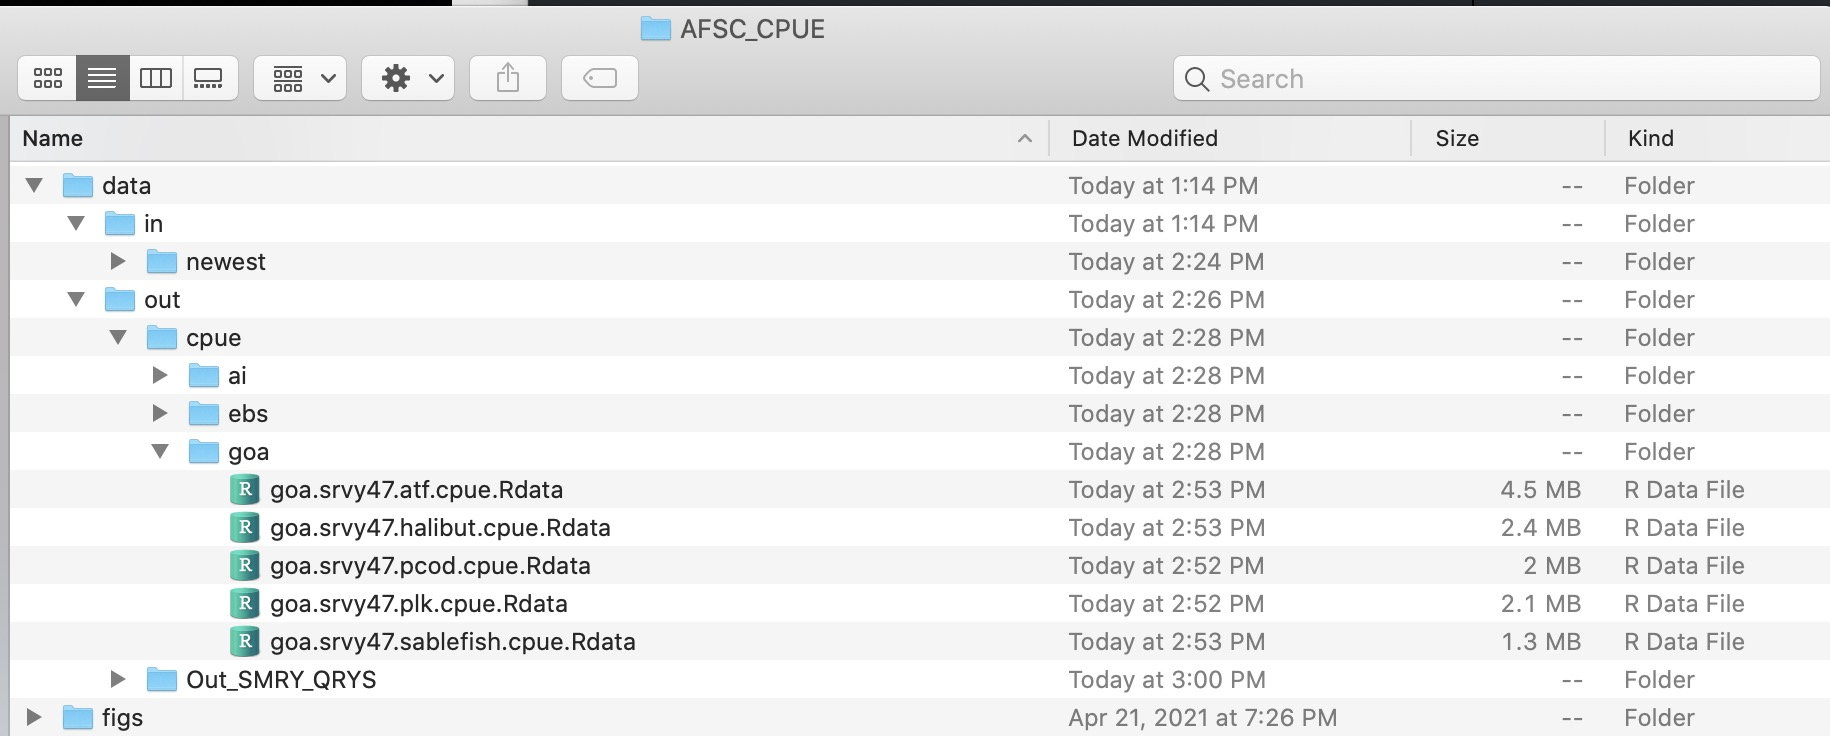
\includegraphics[width=0.9\textwidth,height=\textheight]{figs/out_dir.jpg}
\#\# Step 5: Get annual biomass by age and CEATTLE bins:

\hypertarget{appendix-1-rsetup.rprimary-setup-script}{%
\subsection{\texorpdfstring{Appendix 1: \texttt{R/setup.R}primary setup
script}{Appendix 1: R/setup.Rprimary setup script}}\label{appendix-1-rsetup.rprimary-setup-script}}

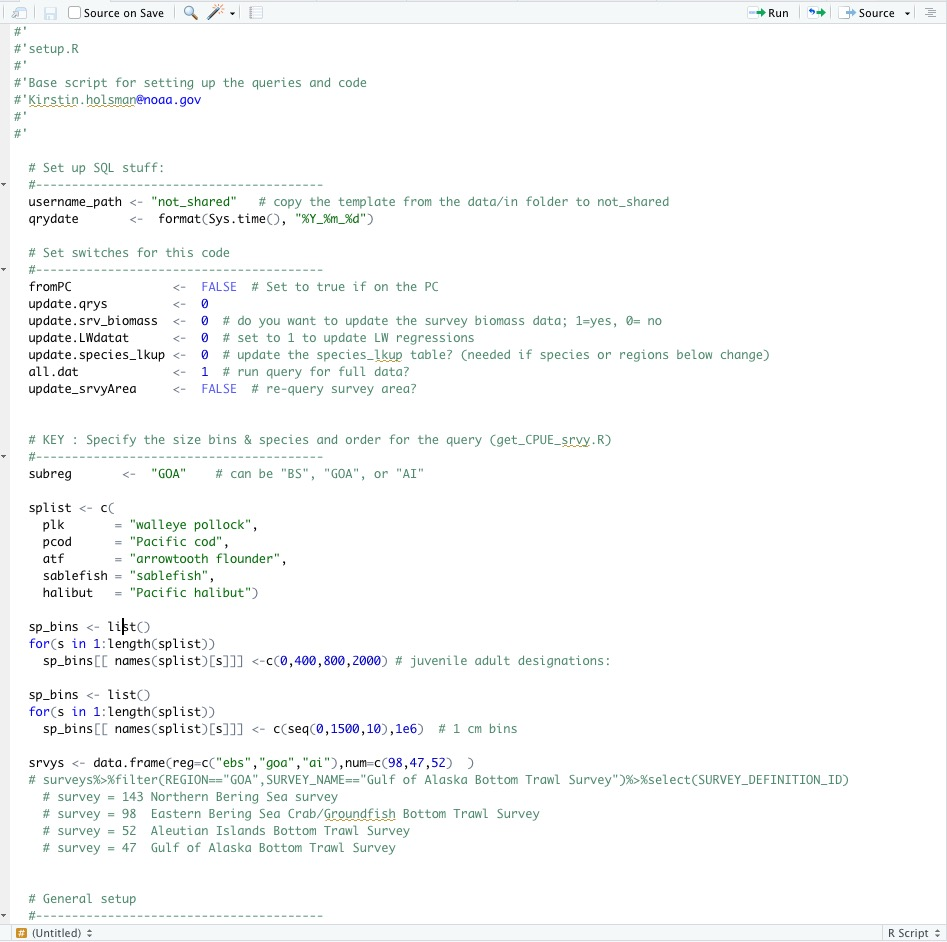
\includegraphics[width=0.9\textwidth,height=\textheight]{figs/setup_large.jpg}

\end{document}
